% ============================================================
%  MANUAL DE USUARIO — Conciliador de Cotizaciones v6.1
%  Compilar con: pdflatex -shell-escape manual.tex
%  Requiere: texlive-full (o MiKTeX completo)
% ============================================================
\documentclass[12pt, a4paper, oneside]{report}

% ── Idioma y codificación ─────────────────────────────────
\usepackage[spanish, es-noshorthands]{babel}
\usepackage[utf8]{inputenc}
\usepackage[T1]{fontenc}

% ── Geometría de página ───────────────────────────────────
\usepackage[
  top=2.5cm, bottom=2.5cm,
  left=3cm,  right=2.5cm,
  headheight=15pt
]{geometry}

% ── Fuentes ───────────────────────────────────────────────
\usepackage{lmodern}
\usepackage{microtype}

% ── Colores corporativos ──────────────────────────────────
\usepackage[dvipsnames, svgnames, x11names]{xcolor}
\definecolor{vino}{HTML}{6E152E}
\definecolor{vinoLite}{HTML}{b84a6b}
\definecolor{darkbg}{HTML}{111217}
\definecolor{panelbg}{HTML}{1d1519}
\definecolor{sidebarbg}{HTML}{2a0f1a}
\definecolor{textMain}{HTML}{f2edf0}
\definecolor{textMuted}{HTML}{d8a8b7}
\definecolor{borderCol}{HTML}{5b2637}
\definecolor{greenOk}{HTML}{28a745}
\definecolor{redWarn}{HTML}{c0392b}
\definecolor{grisClaro}{HTML}{f5f5f5}
\definecolor{grisMedio}{HTML}{dddddd}

% ── Gráficos e imágenes ───────────────────────────────────
\usepackage{graphicx}
\usepackage{float}
\usepackage{caption}
\usepackage{subcaption}

% ── Tablas ────────────────────────────────────────────────
\usepackage{booktabs}
\usepackage{tabularx}
\usepackage{longtable}
\usepackage{array}
\usepackage{multirow}
\usepackage{colortbl}

% ── Cajas de aviso (tcolorbox) ────────────────────────────
\usepackage[most]{tcolorbox}
\tcbuselibrary{breakable, skins}

% Nota informativa
\newtcolorbox{notabox}[1][]{
  enhanced, breakable,
  colback=blue!5!white, colframe=SteelBlue!70!black,
  fonttitle=\bfseries\small, title={Nota},
  left=6pt, right=6pt, top=4pt, bottom=4pt,
  boxrule=0.8pt, arc=4pt, #1
}
% Consejo
\newtcolorbox{consejobox}[1][]{
  enhanced, breakable,
  colback=green!5!white, colframe=greenOk!80!black,
  fonttitle=\bfseries\small, title={Consejo},
  left=6pt, right=6pt, top=4pt, bottom=4pt,
  boxrule=0.8pt, arc=4pt, #1
}
% Advertencia
\newtcolorbox{warningbox}[1][]{
  enhanced, breakable,
  colback=orange!8!white, colframe=orange!80!black,
  fonttitle=\bfseries\small, title={Advertencia},
  left=6pt, right=6pt, top=4pt, bottom=4pt,
  boxrule=0.8pt, arc=4pt, #1
}
% Paso de procedimiento
\newtcolorbox{pasobox}[2][]{
  enhanced,
  colback=vino!6!white, colframe=vino,
  fonttitle=\bfseries\small\color{white},
  title={Paso #2},
  attach boxed title to top left={yshift=-2mm, xshift=4mm},
  boxed title style={colback=vino, arc=3pt},
  left=6pt, right=6pt, top=10pt, bottom=4pt,
  boxrule=0.8pt, arc=4pt, #1
}
% Bloque de código / ruta
\newtcolorbox{rutabox}[1][]{
  enhanced,
  colback=darkbg, colframe=borderCol,
  coltext=textMain,
  fontupper=\ttfamily\small,
  left=8pt, right=8pt, top=4pt, bottom=4pt,
  boxrule=0.6pt, arc=3pt, #1
}

% ── Encabezados y pies de página ──────────────────────────
\usepackage{fancyhdr}
\pagestyle{fancy}
\fancyhf{}
\fancyhead[L]{\color{vino}\small\textbf{Conciliador de Cotizaciones v6.1}}
\fancyhead[R]{\color{gray}\small\leftmark}
\fancyfoot[C]{\color{gray}\small\thepage}
\renewcommand{\headrulewidth}{0.4pt}
\renewcommand{\headrule}{\hbox to\headwidth{\color{vino}\leaders\hrule height\headrulewidth\hfill}}

% ── Hiperenlaces ──────────────────────────────────────────
\usepackage[
  colorlinks=true,
  linkcolor=vino,
  urlcolor=SteelBlue,
  citecolor=vino,
  pdftitle={Manual de Usuario – Conciliador de Cotizaciones v6.1},
  pdfauthor={SHCP - UPIT},
  pdfsubject={Extracción automática de montos en cotizaciones PDF},
  pdfkeywords={cotizaciones, PDF, extracción, IVA, Banxico},
  pdfpagemode=UseOutlines,
  pdfstartview=FitH
]{hyperref}

% ── Listas ────────────────────────────────────────────────
\usepackage{enumitem}
\setlist[itemize]{leftmargin=1.2em, itemsep=2pt}
\setlist[enumerate]{leftmargin=1.4em, itemsep=2pt}

% ── Secciones personalizadas ──────────────────────────────
\usepackage{titlesec}
\titleformat{\chapter}[display]
  {\normalfont\huge\bfseries\color{vino}}
  {\chaptertitlename\ \thechapter}{10pt}{\Huge}
\titleformat{\section}
  {\normalfont\Large\bfseries\color{vino!80!black}}
  {\thesection}{1em}{}
\titleformat{\subsection}
  {\normalfont\large\bfseries\color{vino!70!black}}
  {\thesubsection}{1em}{}

% ── Comandos de utilidad ──────────────────────────────────
\newcommand{\btn}[1]{\texttt{\colorbox{vino!15}{\strut#1}}}
\newcommand{\campo}[1]{\textit{#1}}
\newcommand{\ruta}[1]{\texttt{\small#1}}
\newcommand{\tecla}[1]{\textsf{\small\fbox{#1}}}

% ── Metadata del documento ────────────────────────────────
\title{%
  {\Huge\color{vino}\textbf{Conciliador de Cotizaciones}}\\[6pt]
  {\Large\color{vino!70!black}Manual de Usuario — v6.1}\\[10pt]
  {\normalsize Motor de extracción PDF nativo con PyQt6}
}
\author{SHCP - UPIT}
\date{\today}

% ─────────────────────────────────────────────────────────────
%  INICIO DEL DOCUMENTO
% ─────────────────────────────────────────────────────────────
\begin{document}

% ── Portada ───────────────────────────────────────────────
\begin{titlepage}
  \centering
  \vspace*{3cm}
  {\color{vinoLite}\rule{\linewidth}{2pt}}\\[12pt]
  {\color{vino}\fontsize{36}{44}\selectfont\textbf{Conciliador}}\\[4pt]
  {\color{vino!70!black}\fontsize{18}{24}\selectfont de Cotizaciones}\\[8pt]
  {\color{vinoLite}\rule{\linewidth}{2pt}}\\[20pt]
  {\color{vino!70!black}\Large Manual de Usuario}\\[6pt]
  {\color{vinoLite}\large Versión 6.1}\\[40pt]
  {\color{vino!70!black}\normalsize
    Motor de extracción PDF nativo\\
    5 estrategias de análisis · OCR · API Banxico\\[20pt]
    Interfaz nativa Windows (PyQt6)
  }\\[50pt]
  {\color{borderCol}\small SHCP - UPIT · \today}
\end{titlepage}


\cleardoublepage

% ── Tabla de contenidos ───────────────────────────────────
\tableofcontents
\cleardoublepage

% =============================================================
\chapter{Introducción}
% =============================================================

\section{¿Qué es el Conciliador?}

El \textbf{Conciliador de Cotizaciones v6.1} es una aplicación de escritorio para
Windows que automatiza la extracción y conciliación de montos económicos contenidos
en archivos PDF de cotizaciones de proveedores y presupuestos de proyectos.

Su objetivo es eliminar la transcripción manual de cifras económicas al comparar
documentos PDF con los montos registrados en el Anexo Escrito del proyecto.

\begin{figure}[H]
  \centering
  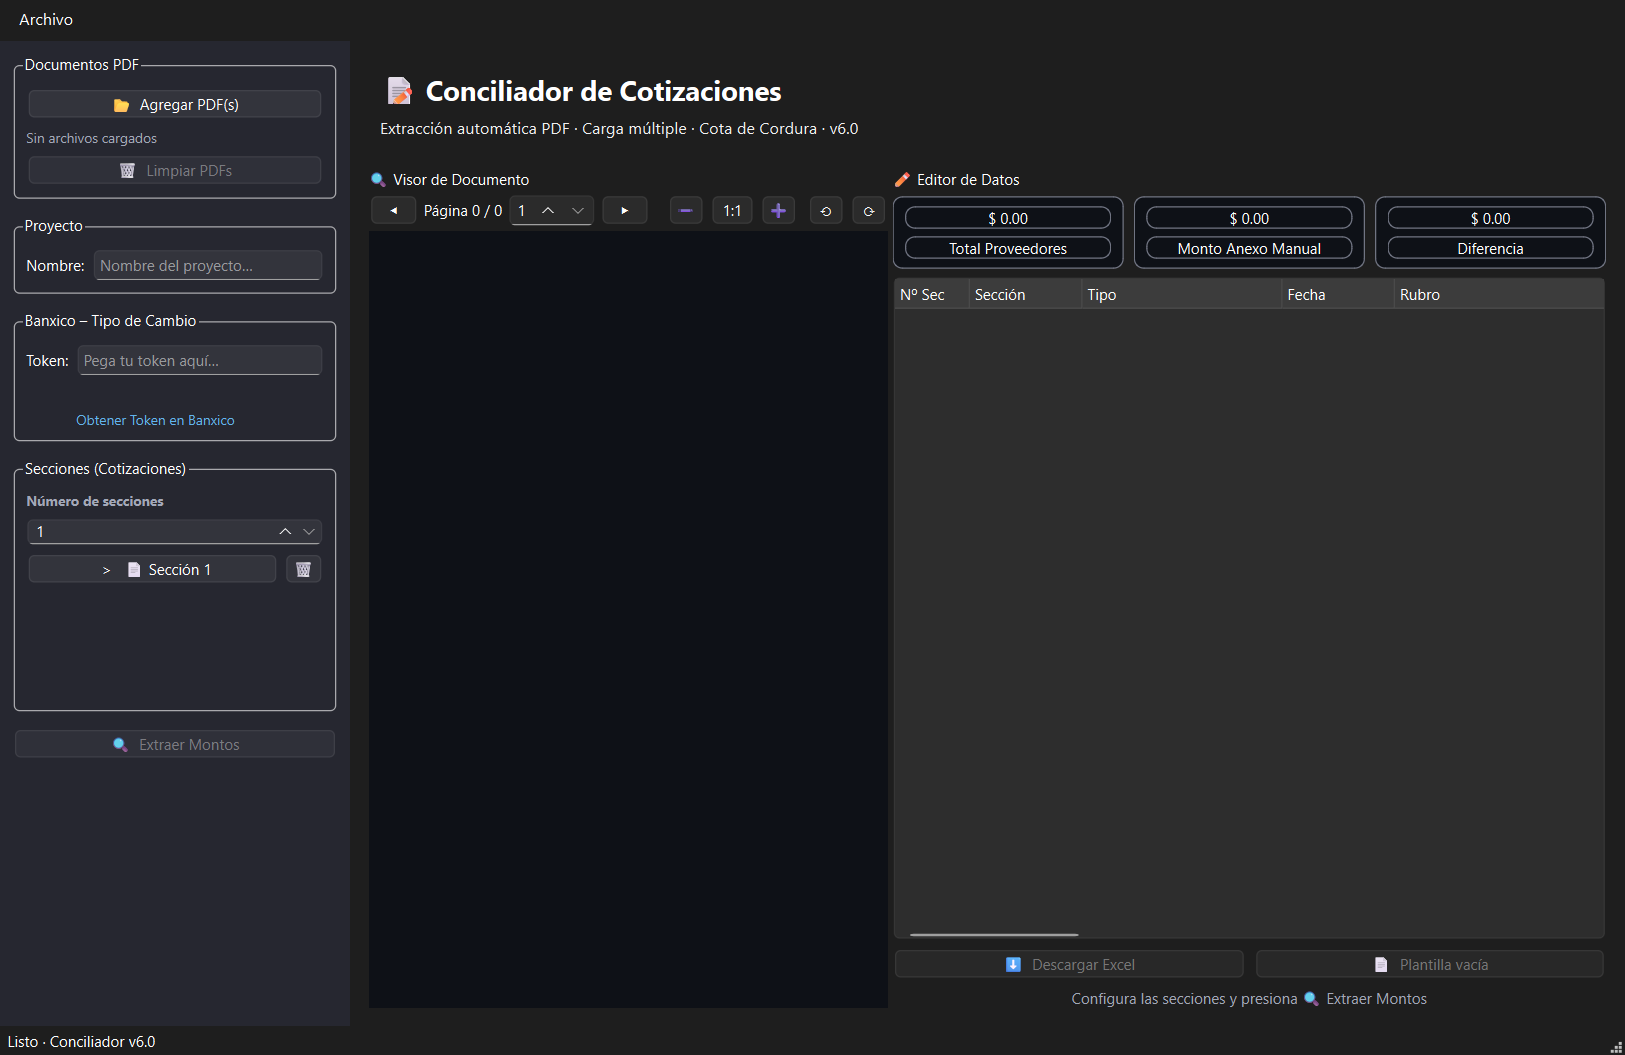
\includegraphics[width=\linewidth]{images/01_estado_inicial.png}
  \caption{Ventana principal del Conciliador — estado inicial al abrir la aplicación.}
  \label{fig:ventana_inicial}
\end{figure}

\section{Características principales}

\begin{itemize}
  \item \textbf{Extracción multinivel:} 5 estrategias independientes de análisis
        (tablas nativas, triangulación, OCR, búsqueda textual y pares adyacentes).
  \item \textbf{Manejo de IVA:} Detecta automáticamente si el IVA está incluido,
        desglosado o exento; descompone el impuesto al 16\%.
  \item \textbf{Conversión de divisas:} Consulta la API del Banco de México (Banxico)
        para obtener el tipo de cambio vigente de USD, EUR y CAD.
  \item \textbf{Multidocumento:} Procesa múltiples PDFs en paralelo, asignando cada
        sección a un archivo y rango de páginas diferente.
  \item \textbf{Exportación a Excel:} Genera un reporte \texttt{.xlsx} con formato
        profesional, fórmulas de validación y estilo corporativo.
  \item \textbf{Interfaz nativa:} Aplicación \texttt{.exe} autónoma para Windows.
\end{itemize}

\section{Público objetivo}

Esta herramienta está diseñada para personal administrativo de EFIDEPORTE
responsable de la conciliación de cotizaciones de proveedores con los montos
contenidos en los anexos escritos de los proyectos deportivos.

% =============================================================
\chapter{Requisitos e Instalación}
% =============================================================

\section{Requisitos del sistema}

\begin{table}[H]
  \centering
  \begin{tabularx}{\linewidth}{lX}
    \toprule
    \textbf{Componente} & \textbf{Requisito mínimo} \\
    \midrule
    Sistema operativo & Windows 10 (64-bit) o superior \\
    Memoria RAM       & 4 GB (recomendado: 8 GB o más) \\
    Espacio en disco  & 500 MB libres (incluye dependencias) \\
    Resolución        & 1280 × 720 px mínimo; 1920 × 1080 recomendado \\
    Conexión a internet & Opcional (solo para tipo de cambio Banxico) \\
    \bottomrule
  \end{tabularx}
  \caption{Requisitos mínimos del sistema.}
\end{table}

\section{Instalación}

La aplicación se distribuye como una carpeta autocontenida generada con
PyInstaller. \textbf{No requiere instalación} — basta con copiar la carpeta y
ejecutar el archivo:

\begin{rutabox}
dist\textbackslash{}Conciliador\textbackslash{}Conciliador.exe
\end{rutabox}

\begin{notabox}
En el primer arranque, Windows Defender SmartScreen puede mostrar el mensaje
``Windows protegió tu equipo''. Haz clic en \textbf{Más información} y luego en
\textbf{Ejecutar de todas formas}. Esto solo ocurre la primera vez.
\end{notabox}

\subsection{Estructura de la carpeta}

\begin{rutabox}
dist\textbackslash{}Conciliador\textbackslash{}\\
\hspace{1em}Conciliador.exe          \textcolor{textMuted}{← ejecutable principal}\\
\hspace{1em}\_internal\textbackslash{}             \textcolor{textMuted}{← dependencias (no modificar)}\\
\hspace{2em}PyQt6\textbackslash{}\\
\hspace{2em}fitz\textbackslash{}\\
\hspace{2em}pandas\textbackslash{}\\
\hspace{2em}...
\end{rutabox}

\begin{warningbox}
No muevas ni elimines la carpeta \texttt{\_internal}. El ejecutable depende de
los archivos que contiene. Mueve siempre la carpeta \texttt{Conciliador}
completa, nunca solo el \texttt{.exe}.
\end{warningbox}

% =============================================================
\chapter{Descripción de la Interfaz}
% =============================================================

La ventana principal está dividida en tres zonas:

\begin{enumerate}
  \item \textbf{Panel lateral} (izquierda): configuración de PDFs y secciones.
  \item \textbf{Visor de PDF} (centro): muestra el documento cargado.
  \item \textbf{Editor de datos} (derecha): tabla de resultados y KPIs.
\end{enumerate}

\section{Panel lateral — Configuración}

\begin{figure}[H]
  \centering
  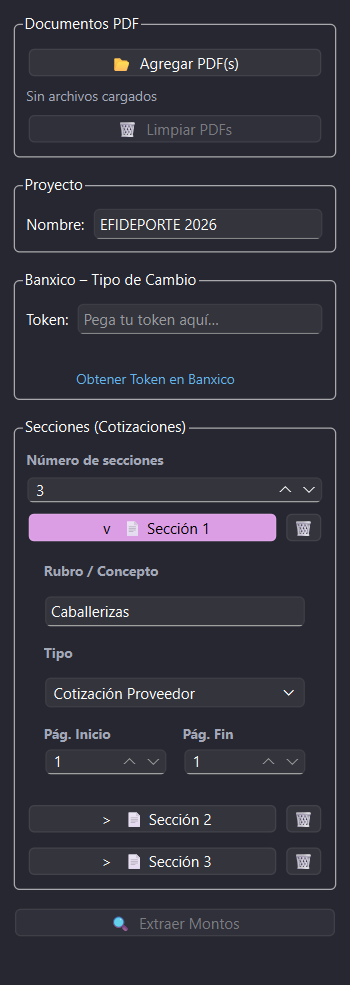
\includegraphics[width=0.32\linewidth]{images/02b_sidebar_zoom.png}
  \caption{Panel lateral con 6 PDFs cargados y 6 secciones configuradas.}
  \label{fig:sidebar}
\end{figure}

El panel lateral contiene cuatro grupos colapsables:

\subsection{Documentos PDF}

\begin{itemize}
  \item \btn{Agregar PDF(s)}: abre el selector de archivos para cargar uno o
        varios PDFs simultáneamente.
  \item \textbf{Lista de archivos}: muestra los archivos cargados con su nombre.
        Si hay más de 3, se puede desplazar con la barra de scroll.
  \item \btn{Limpiar PDFs}: descarga todos los archivos cargados.
\end{itemize}

\subsection{Proyecto}

Escribe el nombre del proyecto (p. ej. ``EFIDEPORTE 2026''). Este nombre aparece
en los encabezados del reporte Excel exportado.

\subsection{Banxico — Tipo de Cambio}

Introduce el token de la API del Banco de México para habilitar la conversión
automática de divisas. El token se muestra enmascarado por seguridad.
Ver \hyperref[sec:banxico]{Sección~\ref{sec:banxico}} para obtener el token.

\subsection{Secciones (Cotizaciones)}

Cada \textbf{sección} corresponde a una cotización o presupuesto que se va a
analizar. Puedes agregar hasta 50 secciones. Para eliminar una sección, haz clic en el botón con ícono de basurero situado junto a su nombre; esto la borrará tanto del panel como de la tabla de resultados automáticamente.

\begin{figure}[H]
  \centering
  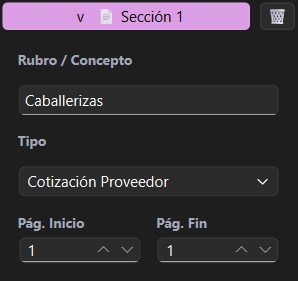
\includegraphics[width=0.45\linewidth]{images/05_seccion_widget.png}
  \caption{Widget de una sección con todos sus campos.}
  \label{fig:seccion_widget}
\end{figure}

\begin{table}[H]
  \centering
  \begin{tabularx}{\linewidth}{lX}
    \toprule
    \textbf{Campo} & \textbf{Descripción} \\
    \midrule
    Rubro & Nombre descriptivo de la cotización (aparece en el reporte). \\
    Tipo  & \textit{Cotización Proveedor} o \textit{Presupuesto Global}.\\
    PDF   & Archivo PDF que contiene esta cotización (visible si hay $>$1 PDF). \\
    Págs. & Rango de páginas a analizar (``De'' y ``A''). \\
    Moneda & MXN, USD, EUR o CAD. Si es diferente a MXN, se convierte. \\
    Detectar IVA & Si está marcado, el motor intenta separar el IVA del total. \\
    Calcular subtotal & Si está marcado, calcula el subtotal sin IVA automáticamente. \\
    \bottomrule
  \end{tabularx}
  \caption{Campos de configuración de una sección.}
\end{table}

\section{Visor de PDF}

El panel central muestra el PDF activo página por página.

\begin{itemize}
  \item \textbf{Paneo y Zoom}: Puedes acercar o alejar el documento. Si el documento tiene zoom, haz clic sostenido y arrastra con el ratón para desplazar la hoja libremente.
  \item \textbf{< / >}: página anterior / siguiente.
  \item \textbf{Spinner de página}: escribe directamente el número de página y
        presiona \tecla{Enter} para saltar.
  \item \textbf{Indicador de sección}: cuando la página cae dentro del rango
        configurado para alguna sección, aparece una etiqueta de color vino
        indicando a qué sección corresponde.
\end{itemize}

\begin{notabox}
El visor solo muestra el PDF; la extracción se realiza en segundo plano por el
motor de análisis, no por lo que se ve en pantalla.
\end{notabox}

\section{Editor de datos}

\begin{figure}[H]
  \centering
  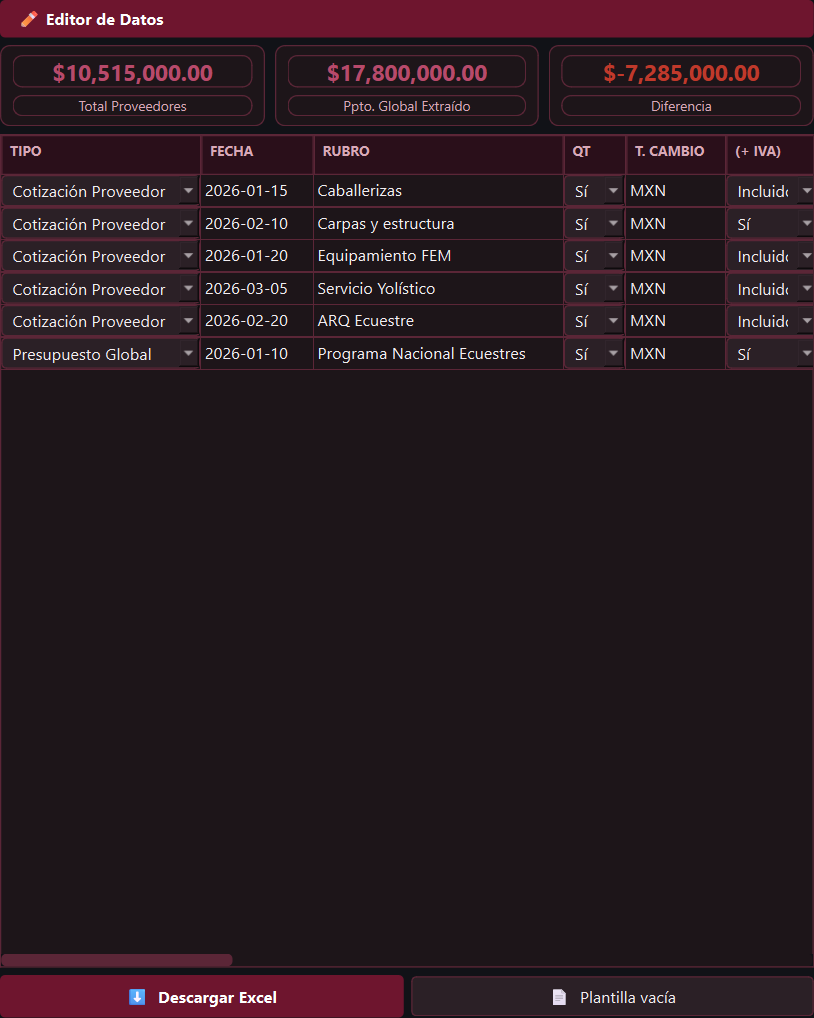
\includegraphics[width=\linewidth]{images/03b_datos_zoom.png}
  \caption{Panel de datos con KPIs y tabla de resultados después de la extracción.}
  \label{fig:datos}
\end{figure}

\subsection{KPIs (indicadores en la parte superior)}

\begin{table}[H]
  \centering
  \begin{tabularx}{\linewidth}{lX}
    \toprule
    \textbf{KPI} & \textbf{Descripción} \\
    \midrule
    Total Proveedores   & Suma de todos los \campo{Total con IVA} de secciones tipo
                          \textit{Cotización Proveedor}. \\
    Monto Anexo Manual  & Suma de los campos \campo{Monto en Anexo Escrito} capturados
                          manualmente; o total del \textit{Presupuesto Global} si existe. \\
    Diferencia          & Total Proveedores $-$ Monto Anexo. \textcolor{greenOk}{Verde}
                          si es cero; \textcolor{redWarn}{rojo} si hay discrepancia. \\
    \bottomrule
  \end{tabularx}
  \caption{Indicadores clave en la parte superior del editor.}
\end{table}

\subsection{Tabla de resultados}

Cada fila corresponde a una sección procesada. Las columnas son editables
directamente — haz doble clic en cualquier celda para modificarla.

\begin{longtable}{lp{0.62\linewidth}}
  \toprule
  \textbf{Columna} & \textbf{Contenido} \\
  \midrule
  \endhead
  Nº Sec             & Número correlativo de la sección para rápida identificación. \\
  Sección            & Nombre de la sección de donde provienen los datos. \\
  Tipo               & Tipo de sección: Cotización o Presupuesto Global. \\
  Fecha              & Fecha detectada en el documento. \\
  Rubro              & Nombre de la sección (configurable). \\
  QT                 & ¿Fue presentada al Comité de Adquisiciones? (Sí/No). \\
  T. Cambio          & Moneda y tipo de cambio aplicado (MXN, USD, EUR, CAD). \\
  (+ IVA)            & Condición del IVA: \textit{Sí}, \textit{Incluido}, \textit{Exento} o \textit{N/M}. \\
  Cantidad           & Número de unidades detectado. \\
  Precio Unitario    & Precio por unidad (sin IVA). \\
  Subtotal (Sin IVA) & Cantidad × Precio Unitario. \\
  IVA 16\%           & Importe del IVA calculado. \\
  Total con IVA      & Total final incluyendo IVA. \\
  Diferencia final   & Total con IVA $-$ Monto en Anexo. \textbf{Calculado automáticamente.} \\
  Monto en Anexo Escrito & Monto registrado en el Anexo del proyecto. \\
  Observaciones      & Notas del motor de extracción y alertas. \\
  \bottomrule
  \caption{Columnas de la tabla de resultados.}
\end{longtable}

% =============================================================
\chapter{Flujo de Trabajo Paso a Paso}
% =============================================================

\begin{figure}[H]
  \centering
  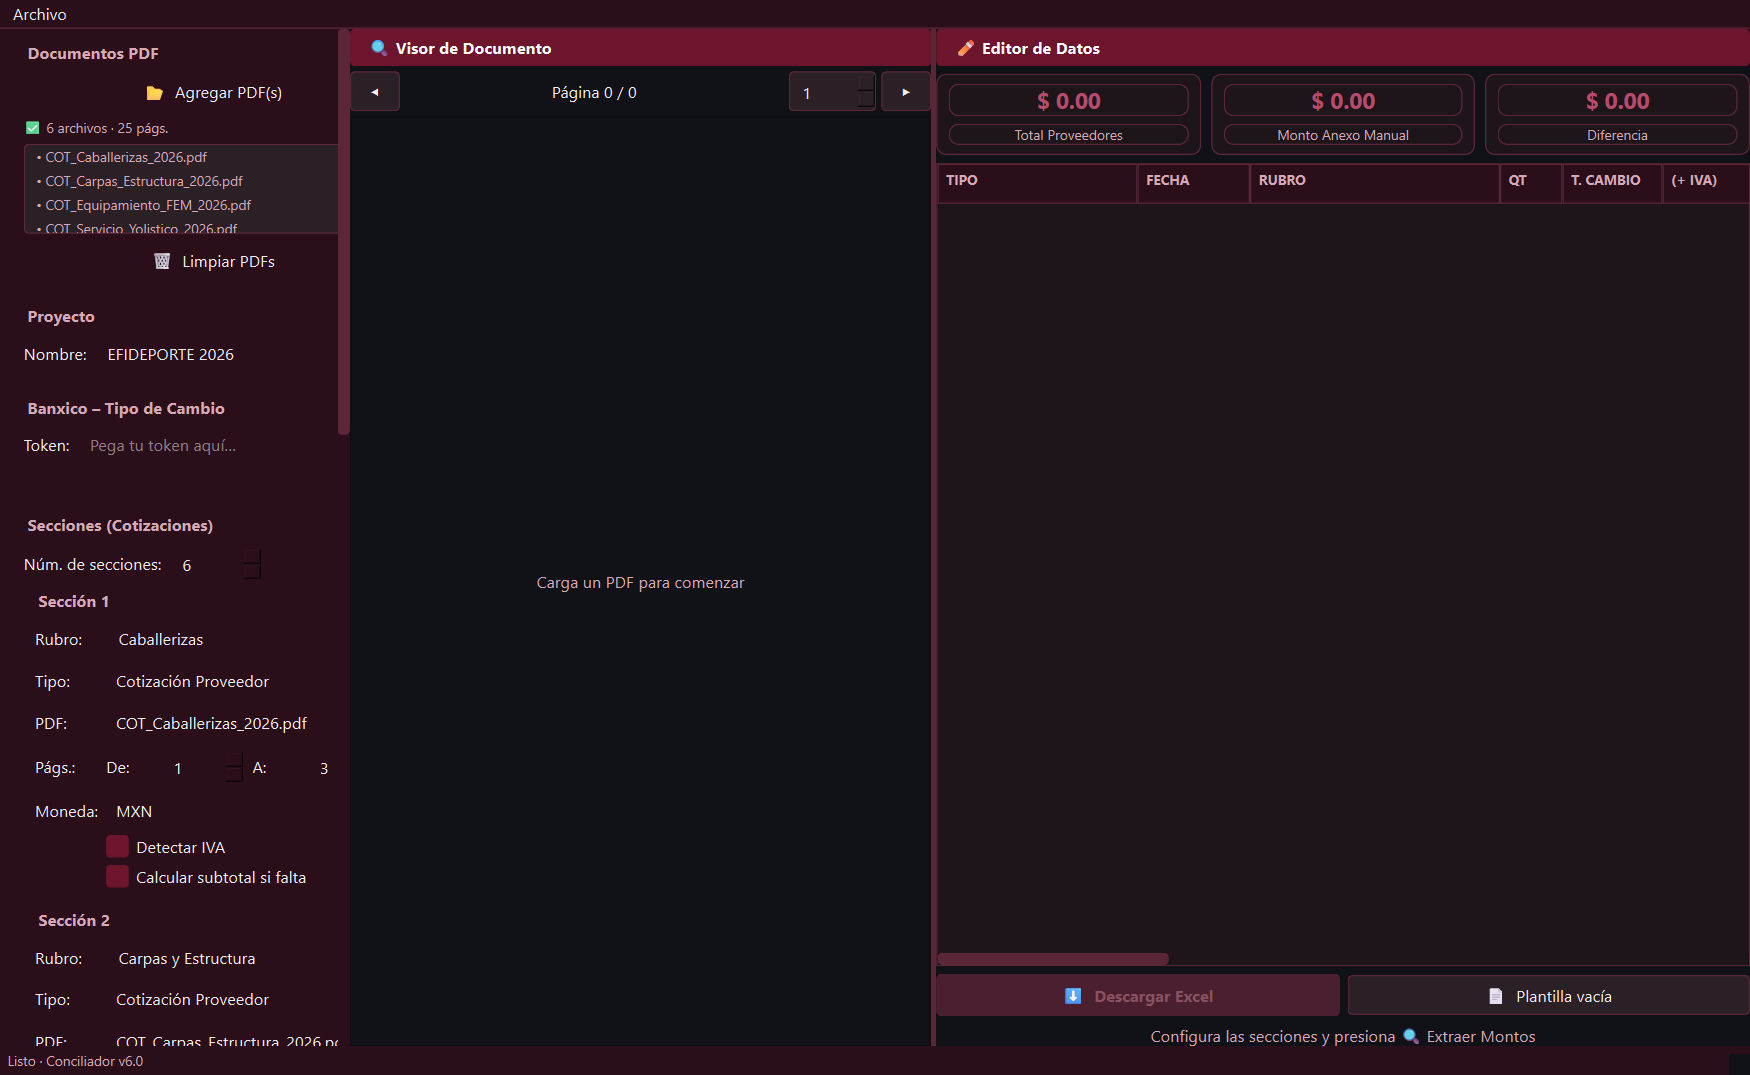
\includegraphics[width=\linewidth]{images/02_sidebar_configurado.png}
  \caption{Aplicación con PDFs cargados y secciones configuradas, lista para extraer.}
  \label{fig:configurado}
\end{figure}

\section{Paso 1 — Cargar los PDFs}

\begin{pasobox}{1}
Haz clic en \btn{Agregar PDF(s)} en la sección \textit{Documentos PDF} del
panel lateral.

\begin{itemize}
  \item Selecciona uno o varios archivos PDF en el explorador.
  \item Para seleccionar varios: mantén presionada \tecla{Ctrl} y haz clic en
        cada archivo, o usa \tecla{Shift} para rangos.
  \item Haz clic en \textbf{Abrir}.
\end{itemize}

La lista de archivos aparece en el panel lateral con el total de páginas.
El PDF se carga automáticamente en el visor central.
\end{pasobox}

\begin{consejobox}
Si las cotizaciones están en documentos separados (un PDF por proveedor),
cárgalos todos a la vez. El sistema los consolida internamente y permite
asignar cada sección a un PDF diferente.
\end{consejobox}

\section{Paso 2 — Escribir el nombre del proyecto}

\begin{pasobox}{2}
En la sección \textit{Proyecto} del panel lateral, escribe el nombre del
proyecto en el campo \campo{Nombre}. Este texto aparecerá en el encabezado
del reporte Excel.

\textbf{Ejemplo:} \texttt{EFIDEPORTE 2026}
\end{pasobox}

\section{Paso 3 — Configurar las secciones}

\begin{pasobox}{3}
\begin{enumerate}
  \item Ajusta el contador \campo{Núm. de secciones} al número de cotizaciones
        o presupuestos que deseas procesar.
  \item Para cada sección:
    \begin{itemize}
      \item Escribe un \campo{Rubro} descriptivo (ej. ``Caballerizas'').
      \item Selecciona el \campo{Tipo} adecuado.
      \item Si cargaste varios PDFs, elige el archivo correspondiente en el
            combo \campo{PDF}.
      \item Establece el rango de páginas (\campo{De} / \campo{A}) donde
            aparece el total de esa cotización.
      \item Selecciona la \campo{Moneda} si no es MXN.
      \item Deja marcado \campo{Detectar IVA} para que el motor determine
            automáticamente si el IVA está incluido o desglosado.
    \end{itemize}
\end{enumerate}
\end{pasobox}

\begin{notabox}
\textbf{¿Cómo sé qué páginas usar?} Navega por el visor PDF con los botones
< / > y revisa dónde aparece el total o tabla de precios de cada cotización.
Anota el número de página (mostrado como ``Página X / Y'') y escríbelo en el
rango correspondiente.
\end{notabox}

\section{Paso 4 — Token Banxico (opcional)}
\label{sec:banxico}

Si alguna cotización está en una moneda diferente a MXN (USD, EUR o CAD),
necesitas un token de la API del Banco de México para obtener el tipo de cambio.

\begin{pasobox}{4}
\begin{enumerate}
  \item Ve a \href{https://www.banxico.org.mx/SieAPIRest/service/v1/token}%
        {www.banxico.org.mx → SIE API → Generar token}.
  \item Resuelve el Captcha de seguridad que solicita la página.
  \item Copia el token generado.
  \item Pégalo en el campo \campo{Token} del panel lateral.
\end{enumerate}
Aparecerá el mensaje \textit{Token activo} cuando el campo tenga contenido.
\end{pasobox}

\begin{warningbox}
Si no proporcionas un token y hay cotizaciones en divisas extranjeras, el
sistema usará la cotización del día anterior almacenada en caché o reportará
el monto en la divisa original sin convertir.
\end{warningbox}

\section{Paso 5 — Extraer los montos}

\begin{pasobox}{5}
Haz clic en el botón \btn{Extraer Montos} (en vino/rojo oscuro) al final
del panel lateral.

\begin{itemize}
  \item La barra de progreso en la parte inferior muestra el avance.
  \item La barra de estado indica qué sección se está procesando.
  \item Al terminar, la tabla de resultados se popula automáticamente.
\end{itemize}
\end{pasobox}

\begin{figure}[H]
  \centering
  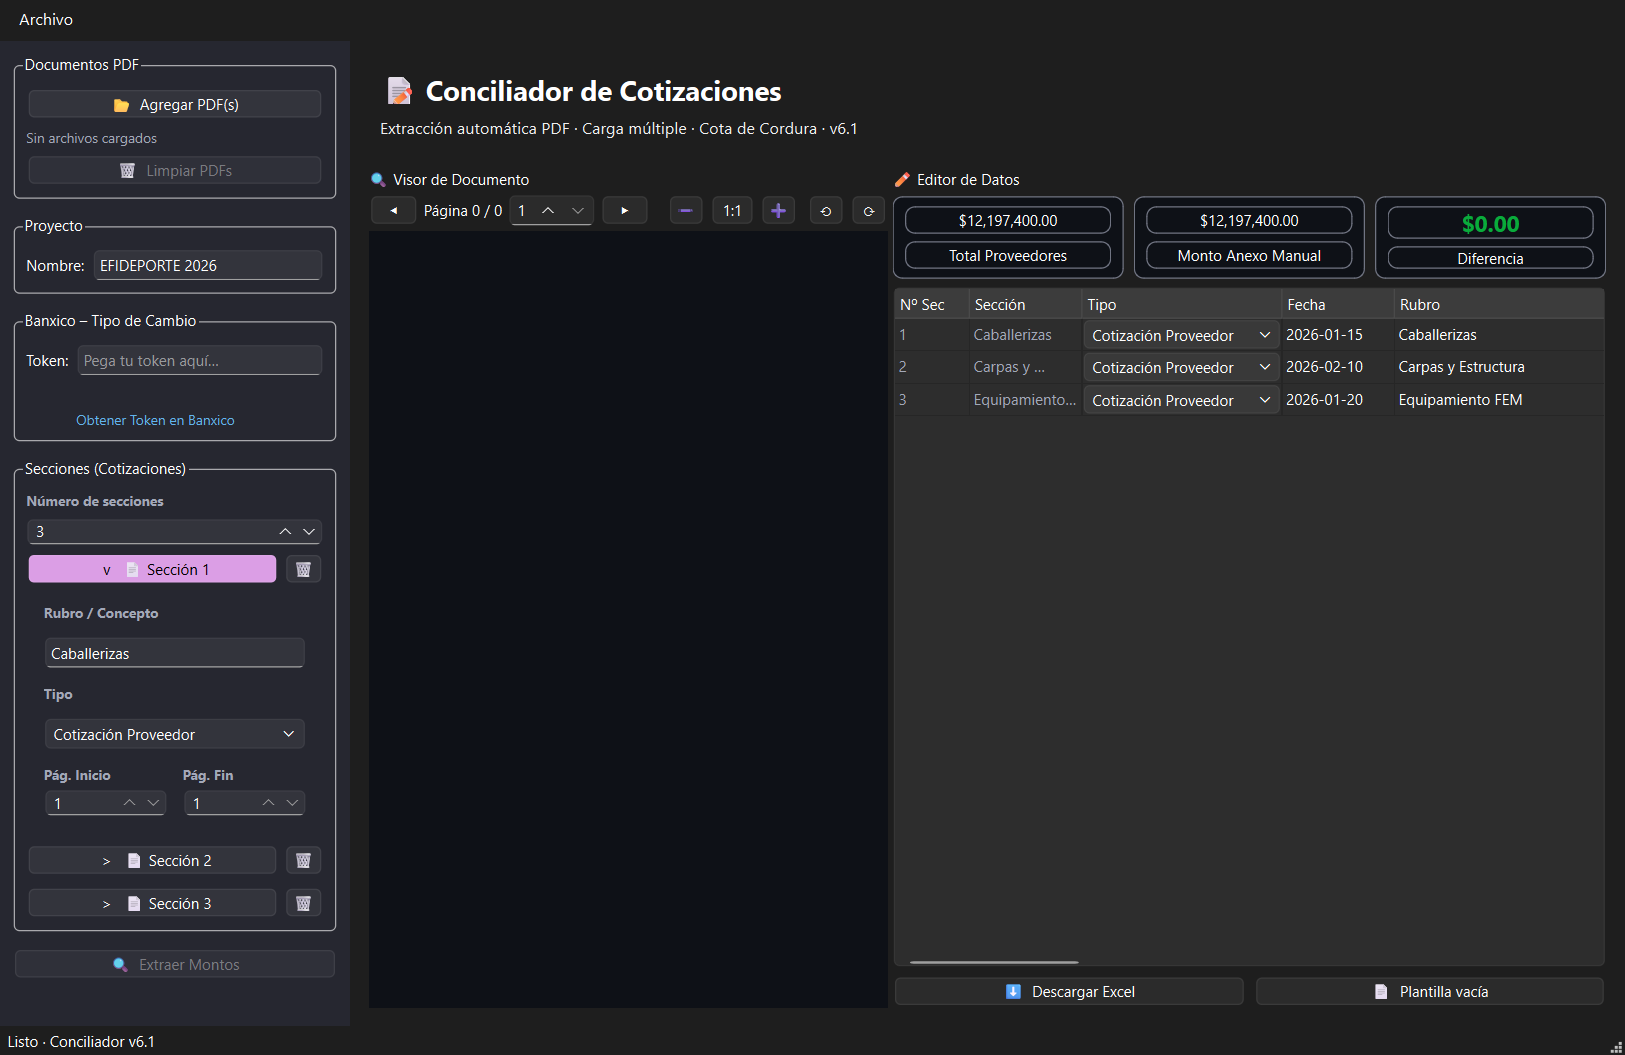
\includegraphics[width=\linewidth]{images/03_tabla_resultados.png}
  \caption{Vista completa después de la extracción: visor PDF + tabla con resultados.}
  \label{fig:resultados}
\end{figure}

\section{Paso 6 — Revisar y ajustar los resultados}

\begin{pasobox}{6}
\begin{enumerate}
  \item Revisa los valores extraídos en la tabla.
  \item Verifica la columna \campo{Observaciones} para entender cómo se obtuvo
        cada monto.
  \item Llena la columna \campo{Monto en Anexo Escrito} con el monto oficial
        registrado en el Anexo del proyecto.
  \item Si algún valor extraído es incorrecto, haz doble clic en la celda y
        corrígelo manualmente.
  \item Las columnas \campo{Diferencia final} y los KPIs se actualizan
        automáticamente al editar cualquier valor.
\end{enumerate}
\end{pasobox}

\begin{notabox}
La columna \campo{Nº Sec}, \campo{Sección} y \campo{Diferencia final} son de solo lectura. La Diferencia final se calcula como
\textit{Total con IVA} $-$ \textit{Monto en Anexo Escrito} y no se puede
editar directamente.
\end{notabox}

\section{Paso 7 — Exportar el reporte}

\begin{pasobox}{7}
\begin{enumerate}
  \item Haz clic en \btn{Descargar Excel} para generar el reporte completo.
  \item Elige la ubicación y nombre del archivo en el diálogo de guardado.
  \item El archivo \texttt{.xlsx} se genera con formato profesional:
    \begin{itemize}
      \item Encabezados en color vino con texto blanco.
      \item Filas alternadas con tono gris claro.
      \item Columnas monetarias con formato \texttt{\$\#,\#\#0.00}.
      \item Fórmulas nativas integradas (Subtotal, IVA, Total, Diferencias) que se recalculan automáticamente si editas los datos.
      \item KPIs de suma al pie de la tabla.
    \end{itemize}
\end{enumerate}

Opcionalmente, \btn{Plantilla vacía} genera el mismo archivo pero sin los
valores numéricos, útil para que un proveedor lo llene manualmente.
\end{pasobox}

% =============================================================
\chapter{Referencia de Campos y Comportamientos}
% =============================================================

\section{Estrategias de extracción}

El motor intenta extraer el monto total en el siguiente orden de prioridad:

\begin{enumerate}
  \item \textbf{Tabla nativa:} Analiza las tablas del PDF y busca la columna
        ``Total''. Toma el valor máximo de la columna (no el primer valor).
  \item \textbf{Triangulación:} Busca tripletas (Cantidad, Precio Unitario, Total)
        que satisfagan $Q \times PU \approx T$.
  \item \textbf{OCR:} Si la página no tiene texto nativo (PDF escaneado),
        aplica reconocimiento óptico de caracteres.
  \item \textbf{Pares adyacentes (G3):} Busca etiquetas como ``Total'',
        ``Importe total'' o ``Es de \$X'' y toma el número más cercano.
  \item \textbf{Búsqueda textual:} Extrae números con patrón monetario
        (\texttt{\$X,XXX.XX}) en contexto de palabras clave financieras.
\end{enumerate}

\section{Tipos de IVA detectados}

\begin{table}[H]
  \centering
  \begin{tabularx}{\linewidth}{lX}
    \toprule
    \textbf{Tipo} & \textbf{Descripción y comportamiento} \\
    \midrule
    Sí        & IVA desglosado en el documento. Se toma el subtotal sin IVA y el total con IVA directamente. \\
    Incluido  & El total ya incluye IVA. El motor descompone: $\text{Sub} = T / 1.16$;
                $\text{IVA} = T - \text{Sub}$. \\
    Exento    & El concepto no causa IVA (ej. servicios médicos, educación).
                IVA 16\% = \$0. \\
    N/M       & No mencionado. El motor no encontró indicación de IVA. Revisa manualmente. \\
    \bottomrule
  \end{tabularx}
  \caption{Tipos de IVA y su comportamiento en el cálculo.}
\end{table}

\section{Conversión de divisas}

Cuando la moneda seleccionada es USD, EUR o CAD:

\begin{enumerate}
  \item El motor consulta la API del Banco de México usando el token configurado.
  \item Obtiene la cotización del día anterior hábil.
  \item Multiplica el monto por el tipo de cambio.
  \item La columna \campo{T. Cambio} muestra la divisa y la tasa usada.
\end{enumerate}

\begin{consejobox}
Los tipos de cambio se almacenan en caché durante la sesión. Si cambias el
token a mitad de sesión, los tipos de cambio ya consultados no se vuelven a
descargar. Reinicia la app para forzar una nueva consulta.
\end{consejobox}

\section{La columna Observaciones}

El campo \campo{Observaciones} es generado automáticamente por el motor de
extracción. Algunos mensajes comunes:

\begin{table}[H]
  \centering
  \begin{tabularx}{\linewidth}{lX}
    \toprule
    \textbf{Mensaje} & \textbf{Significado} \\
    \midrule
    IVA Incluido             & El total encontrado ya tenía IVA; se descompuso al 16\%. \\
    IVA desglosado           & Se encontraron subtotal e IVA separados en el documento. \\
    IVA descompuesto del total & El motor calculó el IVA a partir del total detectado. \\
    Total (línea adyacente)  & El total se tomó de la línea inmediata al renglón con etiqueta ``Total''. \\
    OCR                    & Se usó reconocimiento de caracteres (PDF escaneado); verificar valor. \\
    Error:                   & Falló la extracción; el valor debe capturarse manualmente. \\
    \bottomrule
  \end{tabularx}
  \caption{Mensajes comunes en la columna Observaciones.}
\end{table}

% =============================================================
\chapter{Solución de Problemas}
% =============================================================

\section{La aplicación no arranca}

\begin{itemize}
  \item Verifica que la carpeta \texttt{\_internal} esté junto al ejecutable.
  \item Si aparece el error de SmartScreen, haz clic en \textbf{Más información}
        → \textbf{Ejecutar de todas formas}.
  \item Si el antivirus bloquea la app, agrega una excepción para la carpeta
        \texttt{Conciliador}.
\end{itemize}

\section{No extrae el monto correcto}

\begin{enumerate}
  \item Verifica que el rango de páginas esté correctamente configurado —
        la página donde aparece el total debe estar dentro del rango.
  \item Si el PDF está escaneado (imagen), la extracción depende del OCR.
        La calidad del escaneo afecta el resultado.
  \item Revisa la columna \campo{Observaciones} para entender qué estrategia
        se usó y por qué.
  \item Como último recurso, edita manualmente la celda de \campo{Total con IVA}.
\end{enumerate}

\begin{warningbox}
Los PDFs con tablas complejas, múltiples subtotales o montos en imágenes
incrustadas pueden requerir ajuste manual del rango de páginas o corrección
del valor extraído.
\end{warningbox}

\section{La barra de scroll del panel lateral no aparece}

La barra de desplazamiento vertical del panel lateral aparece automáticamente
cuando el contenido es mayor que la ventana. Si no aparece:

\begin{itemize}
  \item Asegúrate de que la ventana principal tenga al menos 700 px de alto.
  \item Arrastra el borde inferior de la ventana para agrandarla.
\end{itemize}

\section{Error de Token Banxico}

\begin{itemize}
  \item Verifica que el token copiado esté completo (son cadenas largas
        de letras y números).
  \item Los tokens de Banxico tienen vigencia limitada; genera uno nuevo si
        han pasado más de 6 meses.
  \item Sin internet, la consulta fallará silenciosamente y el monto se
        reportará en la divisa original.
\end{itemize}

\section{El archivo Excel no se genera}

\begin{itemize}
  \item Asegúrate de que no haya otro proceso abriendo el archivo de destino.
  \item La ruta de destino debe existir y tener permisos de escritura.
  \item No uses caracteres especiales (\texttt{< > : " / \textbackslash{} | ? *})
        en el nombre del archivo.
\end{itemize}

% =============================================================
\chapter{Preguntas Frecuentes}
% =============================================================

\begin{description}[leftmargin=0pt, style=nextline]

\item[¿Puedo procesar PDFs escaneados?]
Sí, pero la precisión depende de la calidad del escaneo. El motor usa OCR
como estrategia de respaldo. Para mejores resultados, usa PDFs nativos
(generados digitalmente, no escaneados).

\item[¿Cuántos PDFs puedo cargar simultáneamente?]
No hay límite técnico de archivos, pero el procesamiento es secuencial
(una sección a la vez). Con más de 20 PDFs grandes el proceso puede tardar
varios minutos.

\item[¿Qué pasa si dos secciones apuntan al mismo rango de páginas?]
El motor procesa cada sección de forma independiente. Dos secciones pueden
apuntar al mismo PDF y rango; cada una generará su propia fila en la tabla.

\item[¿Puedo editar los datos antes de exportar?]
Sí. Todas las celdas (excepto \campo{Diferencia final}) son editables con
doble clic. Los KPIs y la diferencia se recalculan automáticamente.

\item[¿El programa guarda mis configuraciones?]
La versión actual no guarda la configuración entre sesiones. Debes
reconfigurar las secciones cada vez que abres la aplicación.

\item[¿Funciona sin internet?]
Sí, con la excepción de la consulta del tipo de cambio a Banxico.
La extracción de montos y exportación a Excel funcionan sin conexión.

\item[¿Qué formatos de fecha reconoce?]
El motor detecta fechas en español (``15 de enero de 2026''), formato ISO
(``2026-01-15'') y formato numérico con separadores (``15/01/2026'').

\end{description}

% =============================================================
\chapter{Apéndice Técnico}
% =============================================================

\section{Arquitectura del sistema}

\begin{table}[H]
  \centering
  \begin{tabularx}{\linewidth}{lX}
    \toprule
    \textbf{Módulo} & \textbf{Responsabilidad} \\
    \midrule
    \texttt{engine.py}   & Motor de extracción puro. Contiene toda la lógica de
                           negocio: análisis de PDF, OCR, Banxico, generación de Excel. \\
    \texttt{main\_qt.py} & Interfaz gráfica PyQt6. Gestiona la UI, workers de fondo
                           y comunicación entre componentes. \\
    \bottomrule
  \end{tabularx}
  \caption{Módulos principales de la aplicación.}
\end{table}

\section{Dependencias incluidas}

\begin{table}[H]
  \centering
  \begin{tabularx}{\linewidth}{llX}
    \toprule
    \textbf{Paquete} & \textbf{Versión} & \textbf{Uso} \\
    \midrule
    PyQt6         & $\geq$6.7  & Interfaz gráfica nativa \\
    PyMuPDF       & $\geq$1.24 & Renderizado y extracción de texto PDF \\
    pdfplumber    & $\geq$0.11 & Análisis estructural de tablas PDF \\
    pandas        & $\geq$2.2  & Manipulación de datos tabulares \\
    numpy         & $\geq$2.0  & Operaciones numéricas \\
    openpyxl      & $\geq$3.1  & Generación de archivos Excel \\
    rapidocr      & 1.2.x      & OCR para PDFs escaneados (Python 3.14) \\
    requests      & $\geq$2.31 & Consultas HTTP a la API de Banxico \\
    \bottomrule
  \end{tabularx}
  \caption{Dependencias de la aplicación (incluidas en la carpeta \texttt{\_internal}).}
\end{table}

\section{Expresiones regulares principales}

El motor identifica montos con los siguientes patrones:

\begin{rutabox}
\# Montos con símbolo de peso\\
\$\textbackslash{}s*[\textbackslash{}d,]+(?:\textbackslash{}.\textbackslash{}d\{1,2\})?\\[4pt]
\# Montos con separador de miles (1,234,567.89)\\
(?<!\textbackslash{}d)[\textbackslash{}d]\{1,3\}(?:,\textbackslash{}d\{3\})+(?:\textbackslash{}.\textbackslash{}d\{1,2\})?\\[4pt]
\# Montos decimales sin separador (12345.67)\\
(?<!\textbackslash{}d)\textbackslash{}d\{1,9\}\textbackslash{}.\textbackslash{}d\{2\}(?!\textbackslash{}d)
\end{rutabox}

% ── Contraportada ─────────────────────────────────────────
\clearpage
\thispagestyle{empty}
\pagecolor{white}
\vspace*{\fill}
\begin{center}
  {\color{vino}\rule{0.6\linewidth}{1pt}}\\[12pt]
  {\color{vino}\large Conciliador de Cotizaciones v6.1}\\[6pt]
  {\color{vino}\small Manual de Usuario}\\[6pt]
  {\color{vino}\small SHCP - UPIT · \today}\\[12pt]
  {\color{vino}\rule{0.6\linewidth}{1pt}}
\end{center}
\vspace*{\fill}

\end{document}
